\subsection{Sample storage}
\label{sec:sample-storage}
\noindent The BTO sample was made during one session, stored in the toolbox for the course, and then characterized in a second session. 
The synthesis was done on the 27th of September, and the sample was characterized on the 11th of October.
Unfortunately, the one-inch plastic sample box somehow opened during storage, and the sample was laying loose in the toolbox when it was taken out to be characterized.
% Even though the toolbox is in a cleanroom, the sample was probably exposed to dust and other particles.




\subsection{Optical Images}

\noindent Two images were obatained using an optical microscope.
First, a 5X magnification overview image was taken of one sample corner.
The result of this can be seen in \autoref{fig:optical_overview}.
Then, a 20X magnification image was taken of the middle of the sample.
The result of this can be seen in \autoref{fig:optical_20x}.

\begin{figure}
    \centering
    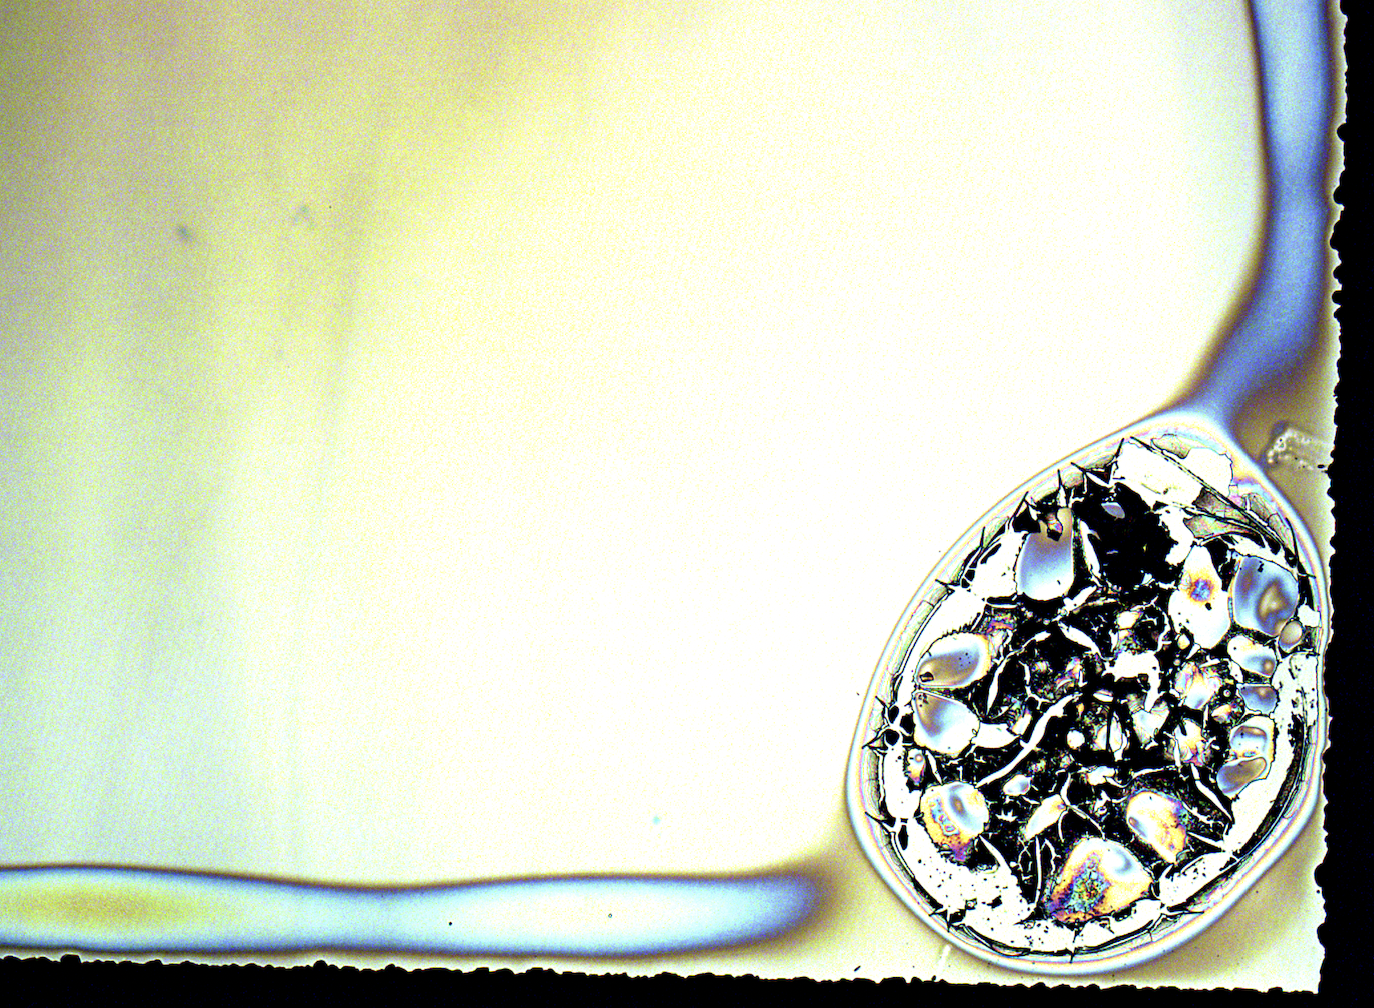
\includegraphics[width=0.45\textwidth]{figures/opt_corner.png}
    \caption{
        Optical overview image of one sample corner.
        The image was taken with a 5X magnification objective.
    }
    \label{fig:optical_overview}
\end{figure}

\begin{figure}
    \centering
    \includegraphics[width=0.45\textwidth]{figures/opt_mid.png}
    \caption{
        Optical 20X magnification image of the middle of the sample.
        The image was taken with a 20X magnification objective.
    }
    \label{fig:optical_20x}
\end{figure}


% profilometer

\subsection{Profilometer}
\label{results:profilometer}

The profilometer data was acquired at three different locations on the sample. 
The data is presented in \autoref{tab:profilometer} and \autoref{fig:profilometer}.
The only data processing done was to center the data around zero, to make the data more comparable.

% table with profilometer data
\begin{table}[ht]
    \centering
    \caption{
    Profilometer data.
    The mean is zero because each data set is centered around zero.
    All measurements are 4000 \textmu m long.
    All numbers are in nm.
    }
    \begin{tabular}{ccccccc}
        Mean &     Median &        STD &        Min &        Max &        Q1 &        Q3 \\
        \hline
        0.00 &      -0.10 &       4.19 &     -11.11 &      50.56 &      -2.54 &       3.17 \\
        0.00 &      -1.04 &       5.75 &     -12.72 &      15.52 &      -4.84 &       4.84 \\
        0.00 &       1.72 &      11.73 &     -21.48 &      29.77 &     -11.77 &       8.44 \\
    \end{tabular}
    \label{tab:profilometer}
\end{table}


% profilometer figure, filename figures/profilometer_graph.jpg

\begin{figure}[ht]
    \centering
    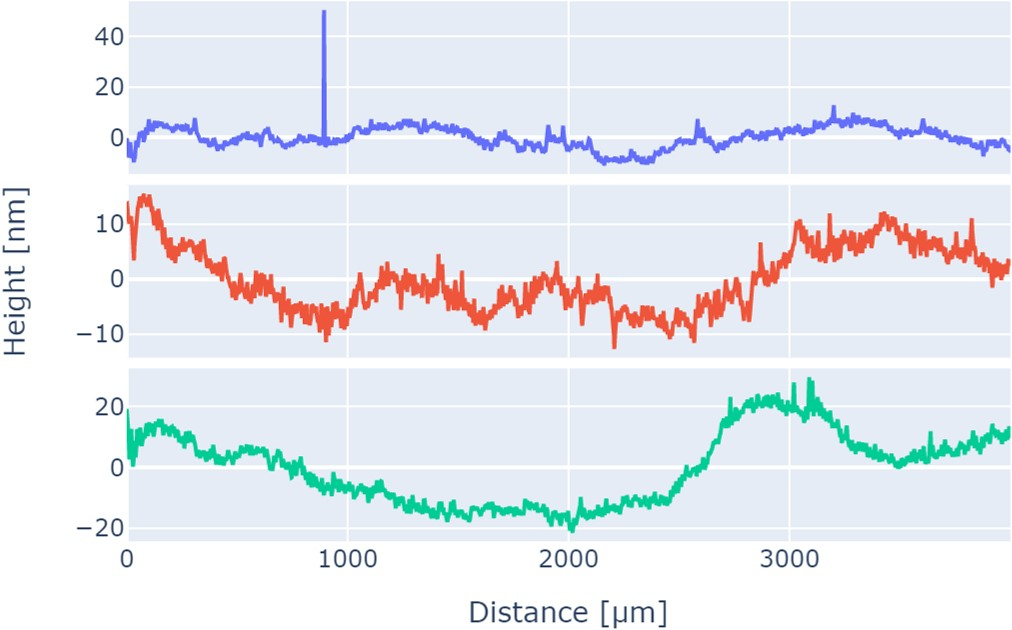
\includegraphics[width=0.45\textwidth]{figures/profilometer_graph.jpg}
    \caption{Profilometer data. 
    Plotted with the mean centered around zero.}
    \label{fig:profilometer}
\end{figure}



% SEM
\subsection{SEM images}
\label{results:SEM}

SEM images were acquired on the SEM APREO at NTNU NanoLab, without coating of the sample.
One of the engineers at NanoLab suggested that the sample would be conductive enough, and showed examples of SEM results from other ferroelectric thin films that were not coated, e.g. \cite{hunnestad_visualizing_2019}.
The examples used low voltage and low current, which was also used in this work.


% SEM image of the corner
\autoref{fig:sem:corner} shows an overview SEM image of a corner, which is the same area in the optical image in \autoref{fig:optical:corner}.
The image was taken with 3 kV and 50 pA, using the EDT detector to get both topography and z-contrast.
The scale bar is 250 \textmu m.


% SEM image of what might be pores
\autoref{fig:sem:pores} shows a closer SEM image of a part of the sample.
The image was taken with 5 kV and 0.1 nA, using the T2 SE detector, thus getting only topography contrast.
The scale bar is 5 \textmu m.


% SEM image filename figures/sem-high-res.jpg
\begin{figure}[ht]
    \centering
    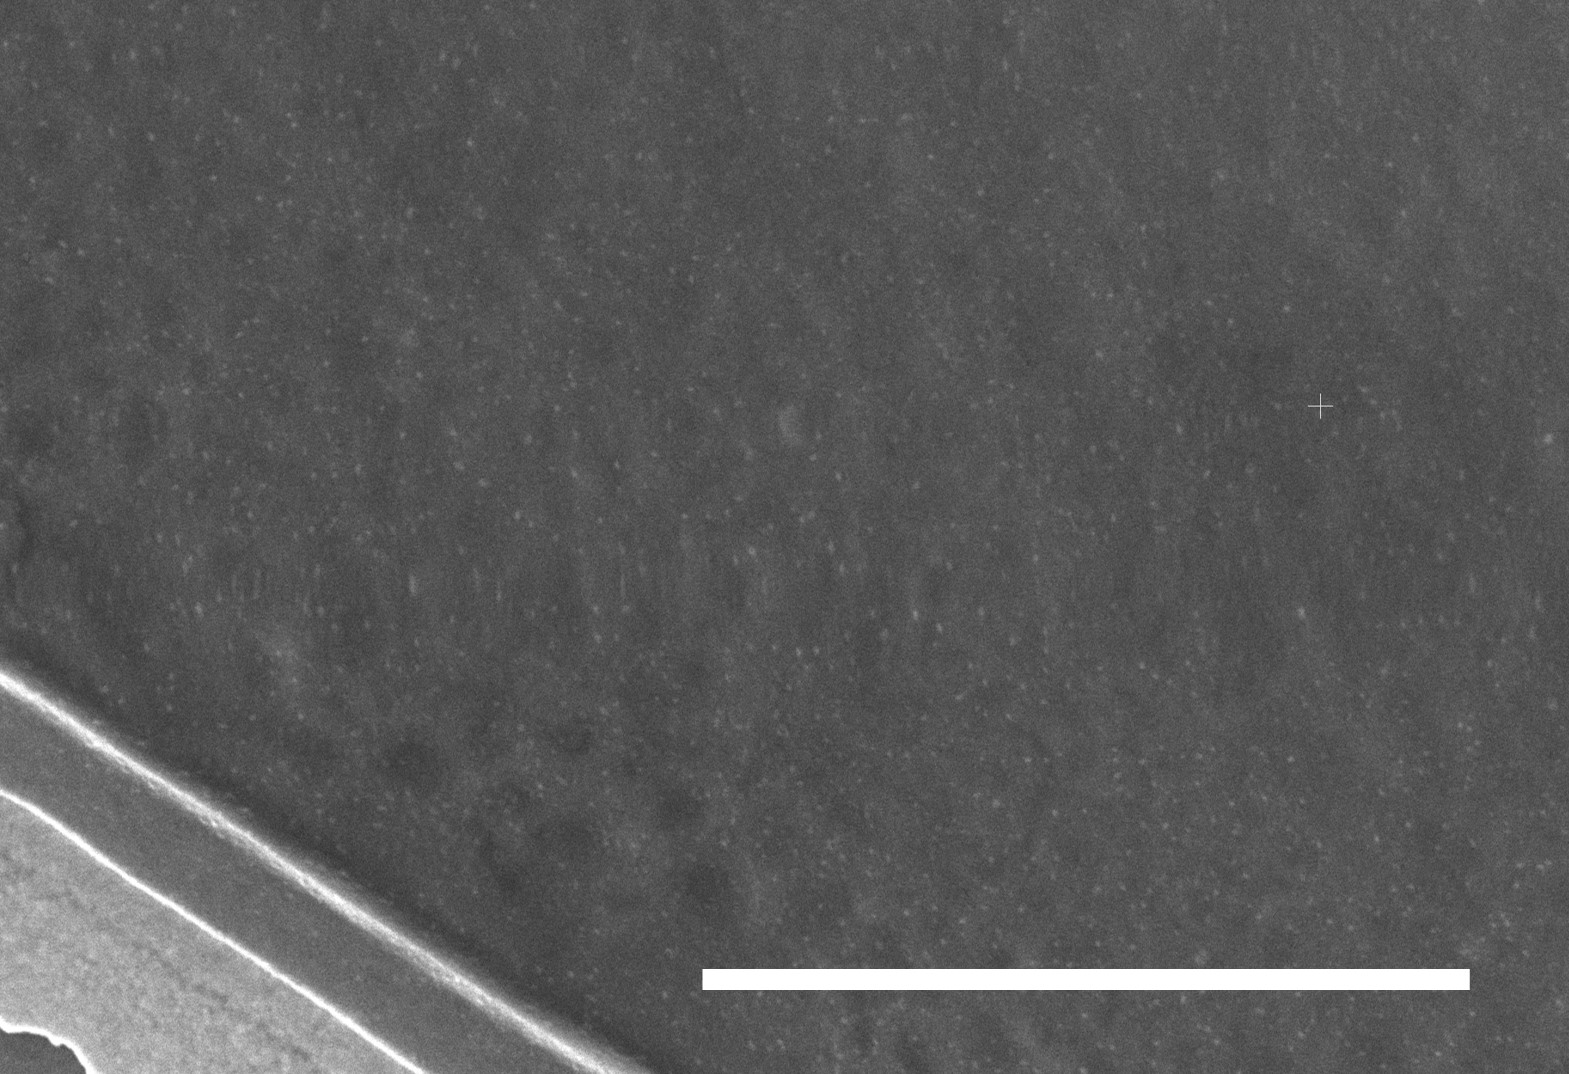
\includegraphics[width=0.45\textwidth]{figures/sem_high_res.jpg}
    \caption{Overview SEM image of a corner of the sample. 
    The scale bar is 250 \textmu m. 
    5 kV, 100 pA, T2 SE detector, 3.0 mm WD. 
    Acquired at NTNU NanoLab.
    }
    \label{fig:sem:corner}
\end{figure}

% SEM image filename figures/sem-overview.jpg
\begin{figure}[ht]
    \centering
    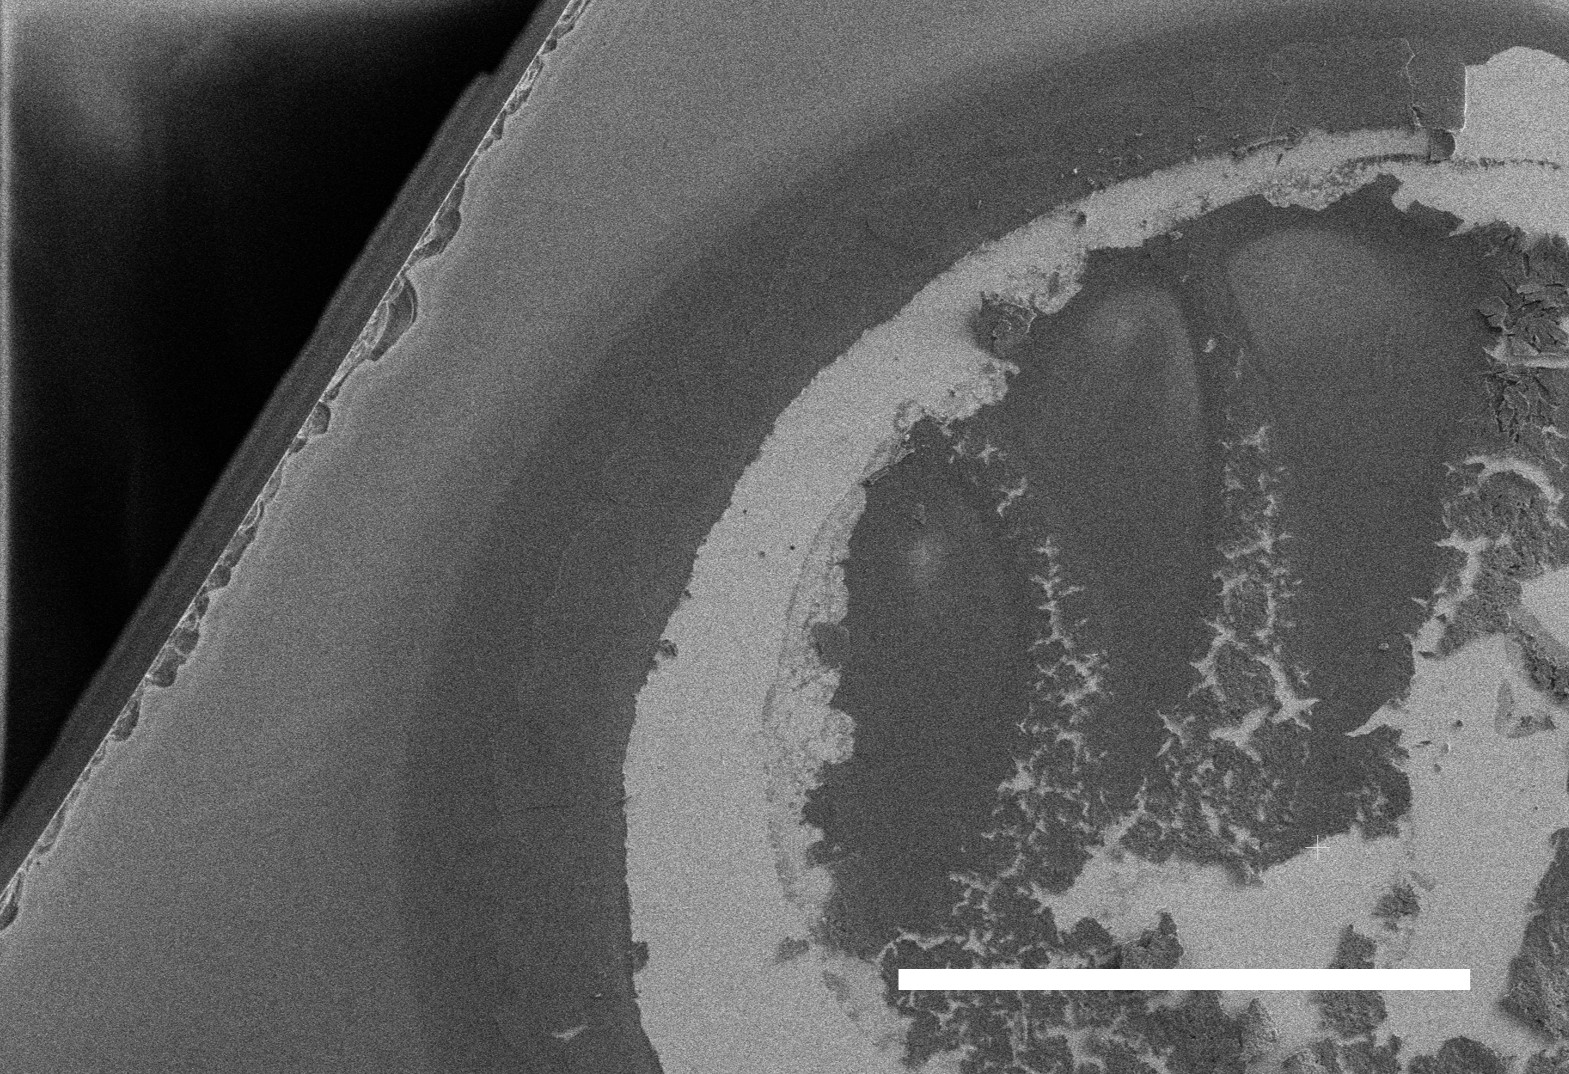
\includegraphics[width=0.45\textwidth]{figures/sem_overview.jpg}
    \caption{Overview SEM image of a part of the sample. 
    The scale bar is 5 \textmu m.
    3 kV, 50 pA, EDT detector, 3.9 mm WD. 
    Acquired at NTNU NanoLab.
    }
    \label{fig:sem:pores}
\end{figure}


